\documentclass[submission, copyright, creativecommons]{eptcs}
\providecommand{\event}{TERMGRAPH 2022} % Name of the event you are submitting to
% \usepackage{breakurl}             % Not needed if you use pdflatex only.
\usepackage{underscore}           % Only needed if you use pdflatex.

% My packages
\usepackage{orcidlink} % Orcid links
\newcommand\Mark[1]{\textsuperscript#1}

\usepackage{subcaption} % Side by side figures
\usepackage{amssymb} % \square command
% Footnotes inside tables
\usepackage{footnote}
\usepackage{glossaries} % Glossary
\makesavenoteenv{tabular}
\makesavenoteenv{table}
\usepackage[nameinlink]{cleveref} % Reference footnotes.
\crefname{figure}{{figure}}{figures}
\Crefname{figure}{{Figure}}{Figures}
\crefformat{footnote}{#2\footnotemark[#1]#3}
% Math
\newtheorem{definition}{Definition}
\newcommand{\definitionautorefname}{Definition}
% Acronyms
\newacronym{bpmn}{BPMN}{Business Process Modeling Notation}

\title{Formalization and analysis of BPMN using graph grammars}
\author{Tim Kräuter\Mark{*}\orcidlink{0000-0003-1795-0611}, \quad
Harald König\Mark{\textdagger}\Mark{*}\orcidlink{0000-0001-6304-6311}, \quad
Adrian Rutle\Mark{*}\orcidlink{0000-0002-4158-1644}, \quad
Yngve Lamo\Mark{*}\orcidlink{0000-0001-9196-1779}
\institute{
\Mark{*}Western Norway University of Applied Sciences, Bergen, Norway
}
\institute{
\Mark{\textdagger}University of Applied Sciences, FHDW, Hannover, Germany}
\email{tkra@hvl.no, harald.koenig@fhdw.de, aru@hvl.no, yla@hvl.no}
}
\def\titlerunning{Formalization and analysis of BPMN using graph grammars}
\def\authorrunning{Kräuter \textit{et al.}}
\begin{document}
\maketitle

% Maximum 8 pages for the first extended abstract(including references)!

\begin{abstract}
The BPMN is a widely used standard notation for defining intra- and inter-organizational workflows to improve the communication between domain experts and software developers.
However, the informal description of the BPMN execution semantics hinders BPMN from reaching its full potential since BPMN constructs are interpreted differently, and behavioral properties cannot be checked.
Consequently, we propose formalizing the BPMN execution semantics based on a model transformation to graph grammars.
Our formalization is one of the most advanced regarding supported BPMN constructs and enables model checking of BPMN-specific and custom properties.
Moreover, we implemented our approach in an open-source web-based tool.
\end{abstract}

\section{Introduction}
% Short Motivation: Formalization of the natural language semantics and model checking
The \gls*{bpmn} is a widely used standard notation to define intra- and inter-organizational workflows to improve the communication between domain experts and software developers.
However, the informal description of the BPMN execution semantics hinders its full adoption \cite{corradiniFormalApproachAnalysis2021, objectmanagementgroupBusinessProcessModel2013}.
Consequently, we propose a new approach to formalize the BPMN execution semantics based on graph grammars.
Our formalization is one of the most advanced regarding supported BPMN constructs and enables model checking of BPMN-specific and custom properties.

The approach is summarized as a BPMN process model in \cref{fig:approach}.
It is based on a model transformation from BPMN process models to graph grammars.
Thus, our approach is \textit{generative}, i.e., it constructs a new graph grammar including rules and a start graph for each BPMN process model.
This is a significant difference compared to other approaches such as \cite{corradiniFormalApproachAnalysis2021, vangorpVisualTokenbasedFormalization2013}, where only the BPMN process model is parsed, but the rewrite rules are fixed.
Generating specific rules for each model leads to possibly more but simpler transformation rules that can be matched faster.
Essentially, complexity is partly shifted from the transformation rules to their generation.

\begin{figure}[h]
    \centering
    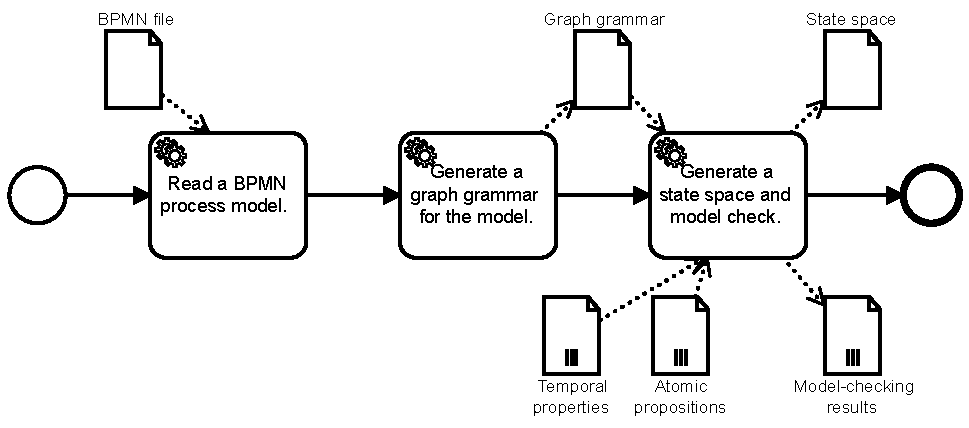
\includegraphics[width=0.6\textwidth]{images/full-approach.pdf}
    \caption{Overview of the proposed approach}
    \label{fig:approach}
\end{figure}

% Paper outline
The remainder of this paper is structured as follows.
First, we describe the semantics formalization using graph grammars (\cref{sec:formalization}) before explaining how this can be utilized for model checking BPMN-specific and custom properties (\cref{sec:modelChecking}).
Then, we shortly present the implementation of our approach resulting in a web-based tool.
Finally, we discuss related work regarding BPMN feature coverage in \cref{sec:relatedWork} and conclude in \cref{sec:conclusion}.

\section{Semantics formalization} \label{sec:formalization}

Since our approach is a model transformation from BPMN to graph grammars, it will generate a \emph{start graph} and \emph{graph transformation rules} for a given BPMN process model (see \cref{fig:bpmnMetamodel}).
However, we only support the BPMN constructs depicted in \cref{fig:bpmnConstructsOverview}.

\begin{figure}[h]
    \centering
    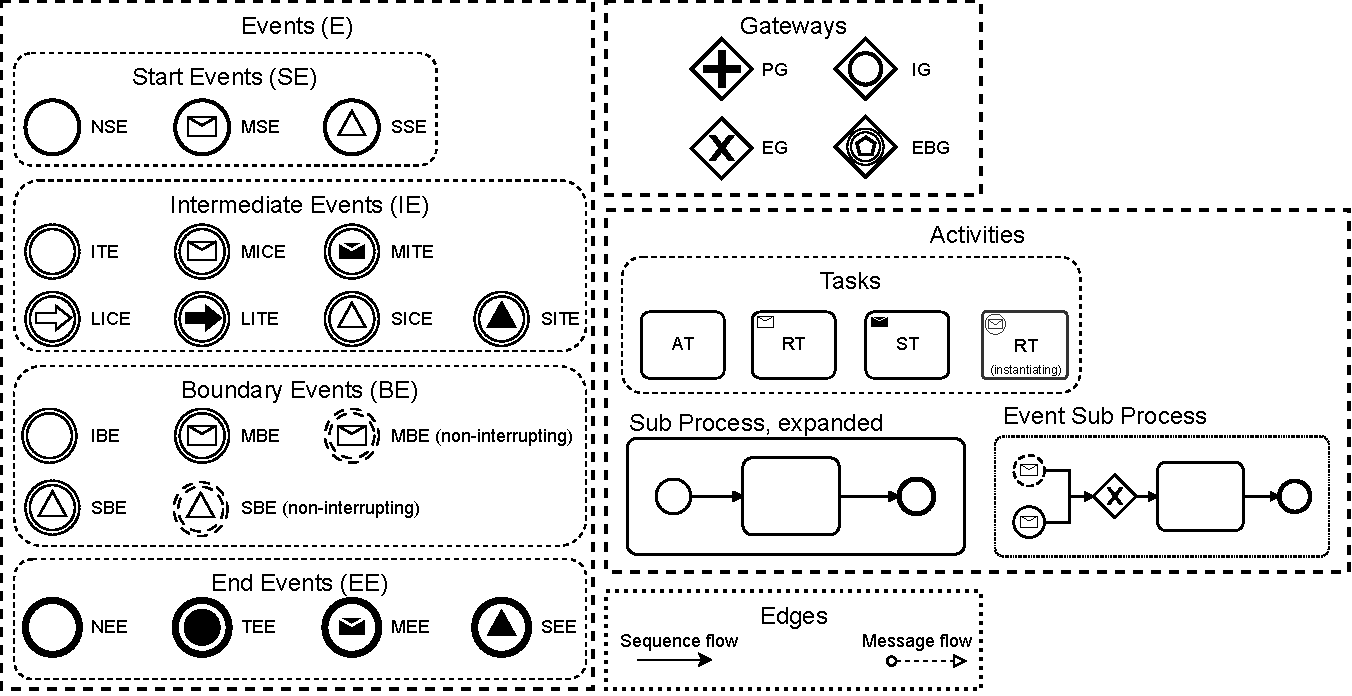
\includegraphics[width=0.8\textwidth]{images/bpmn_semantics-feature_overview.pdf}
    \caption{Overview of the supported BPMN constructs (structure adapted from \cite{houhouFirstOrderLogicVerification2022})}
    \label{fig:bpmnConstructsOverview}
\end{figure}

Our graph-transformation semantics is token-based, as in the informal description of the BPMN specification \cite{objectmanagementgroupBusinessProcessModel2013}.
Thus, to describe processes holding tokens during execution, we use the type graph shown in \cref{fig:typeGraph}.
The type graph is depicted using a UML class diagram-like syntax.

\begin{figure}
\centering
\begin{subfigure}{.5\textwidth}
  \centering
  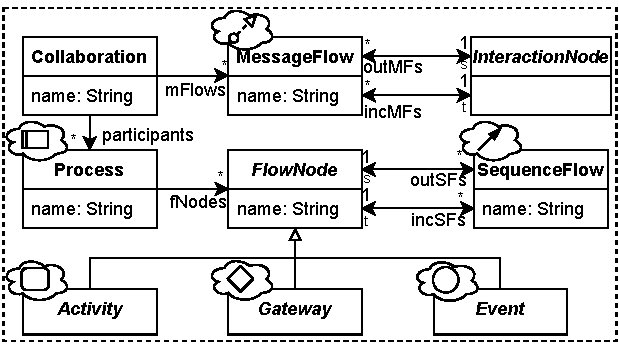
\includegraphics[width=1\linewidth]{images/bpmn_semantics-bpmn-metamodel.pdf}
  \caption{Simplified BPMN metamodel \cite{objectmanagementgroupBusinessProcessModel2013}}
  \label{fig:bpmnMetamodel}
\end{subfigure}%
\begin{subfigure}{.50\textwidth}
  \centering
  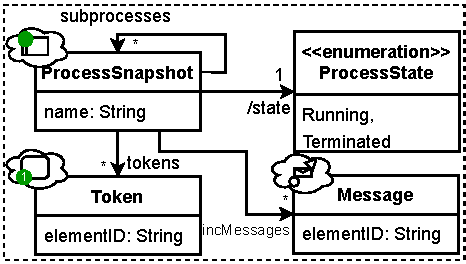
\includegraphics[width=1\linewidth]{images/bpmn_semantics-typegraph.pdf}
  \caption{BPMN execution type graph}
  \label{fig:typeGraph}
\end{subfigure}
\caption{BPMN models}
\label{fig:test}
\end{figure}

We use \textsf{ProcessSnapshot} to denote a running BPMN process with a specific token distribution since it describes one state in the history of process states during the execution.
Every \textsf{ProcessSnapshot} has a set of \textsf{tokens}, incoming \textsf{messages}, and \textsf{subprocesses}.
A \textsf{ProcessSnapshot} has the state \textsf{Terminated} if it has no \textsf{tokens} or \textsf{subprocesses}.
Otherwise, it has the state \textsf{Running}.
A \textsf{Token} has a \textsf{position}, the name (or id in case of identical names) of either a BPMN activity or sequence flow.
A \textsf{Message} has a \textsf{position}, pointing to a message flow.
To depict graphs conforming to the type graph concisely, we introduce a concrete syntax in the clouds attached to the elements.
Tokens are represented as colored circles and are drawn at their specified position in a model.
Their color will match the color of the circle representing the process snapshot holding the token, which is located at the top left of the corresponding BPMN process.
A BPMN pool is depicted as a vertical lane with a name on the left and contains BPMN elements.
Using this type graph, we can now define how the start graph and graph-transformation rules for the different BPMN constructs are created.

% How is a start graph generated?
The generation of the start graph for a BPMN model is straightforward.
For each process in the BPMN model, we generate a process snapshot if the process contains a none start event (NSE).
Then, for each NSE, we add a token to the respective process snapshot.
Furthermore, we consider allowing the user to define a start graph similar to how he can define atomic propositions for custom properties (see \cref{subsec:customProperties}).

We will now describe the rule generation for tasks and message events to overview how our model transformation works.
\Cref{fig:taskRules} depicts the rules generated for a task with two incoming and outgoing sequence flows.
We depict rules with two graphs and a white arrow between them, where the left graph is the prerequisite of the rule application, and the right graph is the result of the rule application.
\begin{figure}[h]
    \centering
    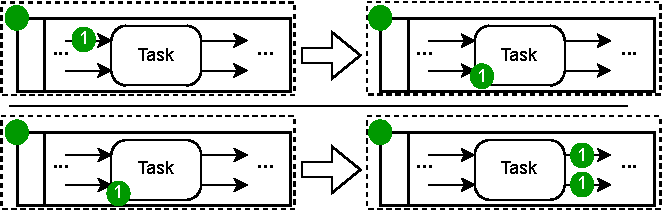
\includegraphics[width=0.65\textwidth]{images/bpmn_semantics-task-rules.pdf}
    \caption{Rules for a task with two incoming and outgoing sequence flows.}
    \label{fig:taskRules}
\end{figure}

The upper rule in \cref{fig:taskRules} represents the start of the task, which will move one token from any incoming sequence flow to the task itself.
The lower rule depicts the execution of the task, resulting in one token on each outgoing sequence flow.
Each graph uses the concrete syntax introduced in \cref{fig:typeGraph}.

The left rule in \cref{fig:messageEventRules} realizes a message throw event, and the right rule implements a message catch event.
The message catch event rule is straightforward, consuming a token and a message and creating an outgoing token.
The message throw event rule moves the token through the event and sends a message to a waiting process snapshot, which must have a token waiting at the corresponding message receive event.
However, sending this message to a different process snapshot is optional.
This can be implemented using nested quantification \cite{rensinkNestedQuantificationGraph2006}.
\begin{figure}[h]
    \centering
    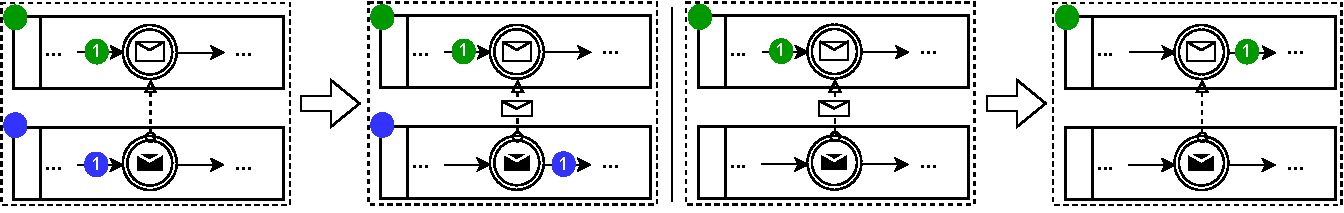
\includegraphics[width=1\textwidth]{images/bpmn_semantics-message-events.pdf}
    \caption{Rules for message intermediate throw/catch events.}
    \label{fig:messageEventRules}
\end{figure}

Process termination is implemented using a general rule applicable to all process snapshots.
The rule is automatically generated once during the model transformation to graph grammars and is used to terminate processes, sub processes, and event sub processes.
It uses negative-application conditions to forbid tokens and sub processes for a process snapshot and then changes its state from running to terminated\footnote{The terminate rule implemented in Groove is contained in the artifacts of this paper \cite{timkrauterArtifactsTERMGRAPH2022}.}.

\section{Model checking BPMN} \label{sec:modelChecking}

Model checking a BPMN process model is straightforward after a graph grammar has been generated.
Besides a graph grammar, a set of temporal properties to be checked and the atomic propositions used in the properties must be supplied (see \cref{fig:approach}).
Atomic propositions are formalized as graphs that can match a state in the state space.
An atomic proposition holds in a state if its graph is a subgraph of the graph representing the state.
This enables model checking of temporal properties using the defined atomic propositions.

Like other work, we differentiate between \emph{BPMN-specific properties} defined generally for all BPMN process models and \emph{custom properties} tailored towards a particular BPMN process model.
We will now give an example of two predefined BPMN-specific properties and how they can be checked using our approach.
Then, we describe how custom properties can be constructed and checked.

\subsection{BPMN-specific properties}
Two BPMN-specific behavioral properties, namely, Safeness and Soundness, are defined in \cite{corradiniClassificationBPMNCollaborations2018}.
Soundness is further decomposed into (i) \emph{Option to complete}: any running process instance must eventually complete, (ii) \emph{Proper completion}: at the moment of completion, each token of the process instance must be in a different end event, (iii) \emph{No dead activities}: any activity can be executed in at least one process instance \cite{corradiniClassificationBPMNCollaborations2018}.
We do not consider structural properties since they can be checked using a standard process modeling tool without implementing execution semantics.
As an example, we will now describe how to implement the \emph{Safeness} and \emph{Option to complete} properties.

% Safe
A BPMN process model is \emph{safe} if, during its execution, at most one token occurs along the same sequence flow \cite{corradiniClassificationBPMNCollaborations2018}.
\emph{Safeness} is checked using the LTL property defined in \eqref{eq:safeness}.
The atomic property \textsf{Unsafe} is true if two tokens of one process snapshot have the same position\footnote{\label{footnote:atomicProps}Groove rules for the atomic properties \textsf{Unsafe} and \textsf{AllTerminated} are contained in the artifacts of this paper \cite{timkrauterArtifactsTERMGRAPH2022}.}.

\begin{align}
    & \square (\neg \,\text{Unsafe}) \label{eq:safeness} \\
    \lozenge (& \square(\text{AllTerminated})) \label{eq:optionToComplete}
\end{align}

% Option to complete
\emph{Option to complete} is checked using the LTL property defined in \eqref{eq:optionToComplete}.
The atomic property \textsf{AllTerminated} is true if there exists no process snapshot in the state running, i.e., all process snapshots are terminated\cref{footnote:atomicProps}.

Both properties can be checked using our implementation \cite{timkrauterArtifactsTERMGRAPH2022}.
To fully check Soundness, the proper completion and no dead activities properties must be checked.
However, the information to check these properties is contained in the state spaces of the generated graph grammars.

\subsection{Custom properties} \label{subsec:customProperties}
% Defining atomic propositions in BPMN is a novelty.
To make model checking user-friendly, we envision users to define atomic propositions in the BPMN syntax, i.e., the concrete syntax introduced earlier.
Thus, to define an atomic proposition, we let the user attach tokens to his BPMN process model, which we can automatically convert to a graph condition.

For example, the token distribution shown in \cref{fig:atomicProposition} defines two running process snapshots with a token in task A.
Differently colored tokens define different process snapshots.
Thus, a user must not be aware of the graph transformation semantics used for execution, which is a significant advantage compared to other approaches.

\begin{figure}[h]
    \centering
    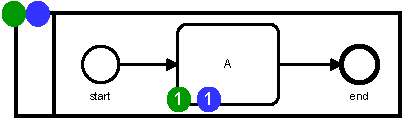
\includegraphics[width=0.35\textwidth]{images/bpmn_semantics-atomicProp.pdf}
    \caption{Token distribution defining an atomic proposition.}
    \label{fig:atomicProposition}
\end{figure}

The token visualization was significantly inspired by the excellent bpmn-js-token-simulation\footnote{\url{https://github.com/bpmn-io/bpmn-js-token-simulation}}.
\section{Implementation} \label{sec:impl}
% Tool
\Cref{fig:implScreenshot} depicts a screenshot of the implemented tool.
The tool is open-source, publicly available, and does not require any installation \cite{timkrauterArtifactsTERMGRAPH2022}.
The tool implements the approach depicted in \cref{fig:approach}.

\begin{figure}[h]
    \centering
    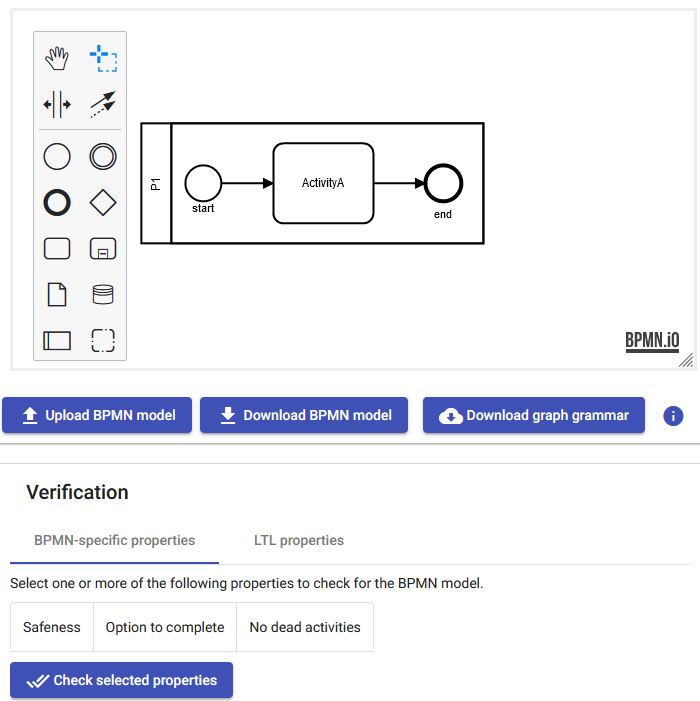
\includegraphics[width=0.6\textwidth]{images/impl.png}
    \caption{Screenshot of the web-based tool}
    \label{fig:implScreenshot}
\end{figure}

Reading and transforming BPMN models to graph grammars is implemented in Java.
Then we use the graph-transformation tool Groove\footnote{\url{https://groove.ewi.utwente.nl/about}} for state space generation and model checking.
% Evaluation
To evaluate the correctness of our implementation, we created a comprehensive test suite, which demonstrates correct rule generation for the implemented BPMN constructs \cite{timkrauterArtifactsTERMGRAPH2022}.

\section{Related work} \label{sec:relatedWork}
% Van gorp
A BPMN formalization based on in-place graph transformation rules is given in \cite{vangorpVisualTokenbasedFormalization2013}.
The formalization covers a substantial part of the BPMN specification, including complex concepts such as inclusive gateway merge and compensation.
In addition, graph transformation rules are visual and thus can easily be matched to the informal description of the execution semantics in the specification \cite{objectmanagementgroupBusinessProcessModel2013}.
The graph transformation rules were implemented in a prototype using GrGen.NET.
Unfortunately, the implementation is not publicly accessible anymore.
Moreover, they do not support model checking since their goal is only formalization.

% BProve/Corradini
The tool BProVe\footnote{\url{http://pros.unicam.it/bprove/}} is based on formal BPMN semantics given in rewriting logic and implemented in the Maude system.
Using these semantics, BProVe enables the verification of custom LTL properties and BPMN-specific properties, such as Safeness and Soundness.
Furthermore, the tool is accessible online, not requiring any installation \cite{corradiniFormalApproachAnalysis2021}.

% fbpmn/Houhou
The verification framework \textsf{fbpmn} uses first-order logic to formalize and check BPMN process models \cite{houhouFirstOrderLogicVerification2022}.
This formalization is then realized in the TLA\textsuperscript{+} formal language and can be model-checked using TLC.
Their framework and related information is open source and freely available online\footnote{\url{https://github.com/pascalpoizat/fbpmn}}.
Similar to BProVe, \textsf{fbpmn} allows checking BPMN-specific properties, such as Safeness and Soundness.
However, they do not allow a user to define custom temporal properties.

We looked in detail at these three approaches since they support a significant subset of the BPMN constructs, have easily accessible and well-documented tool support, and are pretty recent.
Nevertheless, they support a different subset of the BPMN constructs, impacting their usefulness in practice.
\Cref{tab:supportedconstructs} depicts which BPMN constructs are supported by the different approaches compared to our approach.

\begin{table}[htbp]
    \caption{Constructs supported by different BPMN formalizations (overview based on \cite{vangorpVisualTokenbasedFormalization2013}).}
    \label{tab:supportedconstructs}
    \begin{tabular}{l l l l l}
    \hline
      Feature & Van Gorp &  Corradini & Houhou & This\\
      & et al. \cite{vangorpVisualTokenbasedFormalization2013} & et al. \cite{corradiniFormalApproachAnalysis2021}& et al. \cite{houhouFirstOrderLogicVerification2022} & paper\\
      \hline
      \textit{Instantiation and termination} & &\\
      Start event instantiation & X & X & X & X\\
      Exclusive event-based gateway instantiation & X & & & X\\
      Parallel event-based gateway instantiation &  & & & \\
      Receive task instantiation & & & & X\\
      Normal process completion & X & X & X & X\\
      \textit{Activities} & & & &\\
      Activity & X & X & X & X\\
      Subprocess & X & X & X & X\\
      Ad-hoc subprocesses & & & &\\
      Loop activity & X & & &\\
      Multiple instance activity & & & & \\
      \textit{Gateways} & & & &\\
      Parallel gateway & X & X & X & X\\
      Exclusive gateway & X & X & X & X\\
      Inclusive gateway (split) & X & X & X & X\\
      Inclusive gateway (merge) & X & & X & X\\
      Event-based gateway &  & X\footnote{Does not support receive tasks after event-based gateways.} & X & X\\ % No timer and conditional events after event based gateway supported.
      Complex gateway & & & &\\
      \textit{Events} & & & & \\
      None Events & X & X & X & X\\
      Message events & X & X & X & X\\
      Timer Events & & & X & \\
      Escalation Events & & & & \\
      Error Events (catch) & X & & &\\
      Error Events (throw) & X & & &\\
      Cancel Events & X & & &\\
      Compensation Events & X & & &\\
      Conditional Events & & & &\\
      Link Events & X & & & X\\
      Signal Events & X & & & X\\
      Multiple Events &  & & & \\
      Terminate Events & X & X & X & X\\
     Boundary Events & X\footnote{Only supports interrupting boundary events on tasks.} & & X\footnote{Only supports message and timer events.} & X\\ % To the same extent as the event support
      Event subprocess &  &  &  & X\\
    \end{tabular}
\end{table}

% Summarize the findings and explain them in more detail
% Explain Van Gorp in detail
Van Gorp et al. \cite{vangorpVisualTokenbasedFormalization2013} cover a large part of the BPMN semantics.
However, they do not support Event-based gateways and event subprocesses, while their support for boundary events is minimal.
Especially, Event-based gateways are often used and supported by every other approach.
% Explain Corradini in detail
Corradini et al. \cite{corradiniFormalApproachAnalysis2021} does only support message and terminate events.
However, many other types of events exist and are used in practice.
% Explain Houhou in detail
In addition to \cite{corradiniFormalApproachAnalysis2021}, Houhou et al. \cite{houhouFirstOrderLogicVerification2022} support timer and the use of message and timer events as both interrupting and non-interrupting boundary events.
However, the support of different event types remains limited compared to \cite{vangorpVisualTokenbasedFormalization2013}.

Referring to \cref{tab:supportedconstructs}, we conclude that our formalization is comprehensive but still lacks support for some of the more advanced event types.
An implementation of the missing event types is feasible, as shown in \cite{vangorpVisualTokenbasedFormalization2013}.

\section{Conclusion \& future work} \label{sec:conclusion}
% Summary
We presented a formalization of the BPMN execution semantics based on a model transformation to graph grammars.
Thus, complexity shifts from the graph transformation rules to the model transformation when compared to fixed graph transformation rules.
% Formalization & model checking
Our resulting BPMN formalization is comprehensive and supports model checking.
% Tool
In addition, we started implemented our approach in a web-based tool to make our ideas easily accessible to other researchers and potentially practitioners in the future.

% Future work
We aim to improve our formalization and resulting tool in multiple ways in the future.
% More semantics
First, we intend to extend our formalization to support even more BPMN constructs for example error, cancel and compensation events.
% Proper evaluation
Second, we plan to evaluate our approach on syntactical models and on models from open repositories such as the "BPM Academic Initiative Model Collection" \cite{weskeModelCollectionBusiness2020} and "Camunda BPMN for
Research"\footnote{\url{https://github.com/camunda/bpmn-for-research}}.
% Implementing the atomic proposition definition
Third, we want to extend the features of our tool.
One should be able to define atomic propositions for model checking in the tool directly, as described in \cref{sec:modelChecking}.
% Counterexample simulation like Houhou
Furthermore, counterexamples found during model checking should be visualized directly in the tool, like the implementation in \cite{houhouFirstOrderLogicVerification2022}, such that users must not understand the underlying implementation in Groove.
\bibliographystyle{eptcs}
\bibliography{bib}
\end{document}
